\documentclass{article}

\usepackage{scribe}

\setseriestitle{Probabilistic Machine Learning and Inference}
\setscribecode{2}
\setauthname{Gurpreet Singh}
\setinstrname{Piyush Rai}
\setheaddate{December 2, 2017}
\settitle{Parameter Estimation in Probabilistic Models}

\begin{document}
\makeheader

\begin{ssection}{Point Estimate}

	Point estimate is a computationally cheaper alternative to fully Bayesian Inference. It gives the single best estimate to an optimization problem. There are two types of Point Estimates -- Maximum Likelihood Estimation (MLE) and Maximum-a-Posteriori (MAP)

	\begin{ssubsection}{Point Estimation via MLE}

		MLE finds the estimate that maximizes the log-Likelihood $\para{\log{\prob{\vX \pipe \vtheta}}}$. We can write the maximization function as

		\begin{align*}
			\lagr{\vtheta}	\eq	\log{\prob{\vX \pipe \vtheta}}
		\end{align*}

		If the data points are independent, we can write this the joint probability as

		\begin{align*}
			\prob{\vX \pipe \vtheta}		&\eq	\prod_{n = 1}^N \prob{\vx^n \pipe \vtheta} \\
			\implies \lagr{\vtheta}	&\eq	\sum_{n = 1}^N \log{\prob{\vx^n \pipe \vtheta}}
		\end{align*}

		\begin{figure}[h!]
			\centering
			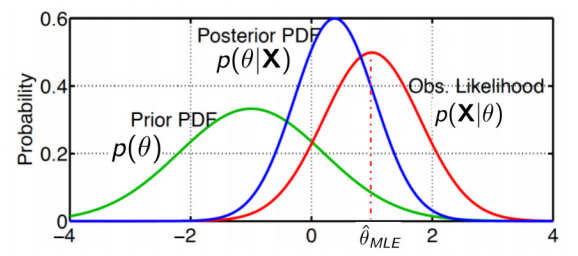
\includegraphics[width=250px]{includes/scribe02/mle-estimate.png}
			\caption{Visual Look at MLE Estimate}
		\end{figure}

		\note{MLE is consistent, i.e. as N $\lra \infty$ the value of $\widehat{\vtheta}_{MLE}$ converges to the real $\vtheta$}

	\end{ssubsection}

	\begin{ssubsection}{Point Estimate via MAP}

		MAP finds the estimate that maximizes the log-posterior-probability $\para{\log{\prob{\vtheta \pipe \vX}}}$. We can write the maximization function as

		\begin{align*}
			\lagr{\vtheta}	&\eq	\log{\prob{\vtheta \pipe \vX}} \\
									&\eq	\log{\prob{\vX \pipe \vtheta}} + \log{\prob{\vtheta}}
		\end{align*}

		Again, if the data points are independent, we can write

		\begin{align*}
			\prob{\vX \pipe \vtheta}		&\eq	\prod_{n = 1}^N \prob{\vx^n \pipe \vtheta} \\
			\implies \lagr{\vtheta}	&\eq	\sum_{n = 1}^N \para{\log{\prob{\vx^n \pipe \vtheta}}} + \log{\prob{\vtheta}}
		\end{align*}

		\begin{figure}[h!]
			\centering
			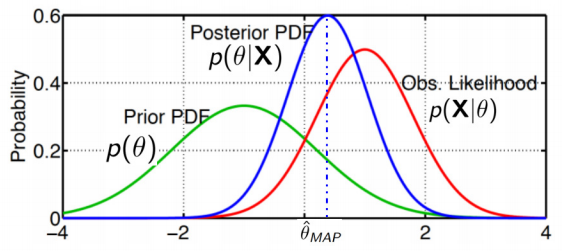
\includegraphics[width=250px]{includes/scribe02/map-estimate.png}
			\caption{Visual Look at MAP Estimate}
		\end{figure}

		\note{When the prior is uniform, the MLE and MAP estimates are the same}

		MAP estimate is not Bayesian, as it still gives a point estimate (can be considered as optimization with regularization). We are still not modelling the uncertainty in the parameter estimation.

	\end{ssubsection}

	\begin{ssubsection}{Point Estimate via Loss Minimization Function}

		Instead of maximizing the log-probability, we can also minimize the negative-log-probability. This is the loss function. \br

		In case of both MLE and MAP, the loss function is the NLL (Negative Log Likelihood). For MLE, we minimize the following function

		\begin{align*}
			\func{\mt{L}}{\vtheta}	\eq	\func{\mt{NLL}}{\vtheta}	\eq	-\log{\prob{\vX \pipe \vtheta}}
		\end{align*}

		In case of MAP, we minimize the loss function with a regularizer term

		\begin{align*}
			\tfunc{L}{\vtheta}	\eq	\tfunc{NLL}{\vtheta} - \log{\prob{\vtheta}}
		\end{align*}

		\note{NLL is the `loss function' and $-\log{\prob{\vtheta}}$ is the regularizer term} \br

		Thus, MLE is like emperical risk / loss minimization (ERM) and MAP is like regularized ERM.

	\end{ssubsection}

	\begin{ssubsection}{Point Estimate Example: Coin-Toss}

		Consider a simple problem. We toss a coin $N$ times. The task is to predict the next outcome. Assume consecutive coin tosses to be independent. \br

		Say the outcome of toss is oru random variable $x$. Since there are two options, the logical choice is a Bernoulli distribution. Hence we can write the probability function of the random variable $x \in \set{0, 1}$ (where 1 represents `Head' and 0 represents `Tail') conditioned on the bias $\theta$ as follows

		\begin{align*}
			\prob{x}	\eq	\theta^{x} \para{1 - \theta}^{1 - x}
		\end{align*}

		Since this is the probability of our data points, we can write the log-likelihood as follows

		\begin{align*}
			\log{\vX \pipe \theta}	\eq	\sum_{n = 1}^N x^n \log{\theta} + \para{1 - x^n} \log{1 - \theta}
		\end{align*}

		Maximizing the log-likelihood, we get the MLE estimate $\para{\wtheta_{MLE}}$

		\begin{align*}
			\wtheta_{MLE}	\eq	\frac{\sum_{n = 1}^N x^n}{N}
		\end{align*}

		In this case, MLE is simply the fraction of heads. The problem with MLE is that it does not express our prior beliefs about $\theta$. This can be problematic if the number of samples is very less (the number of heads might be zero) \br

		To avoid this, we use the MAP estimate. Here, we are faced with another problem of inductive bias. We need to choose the prior distribution. In our case, we need to find a probability function for the random variable $\theta$. \br

		Since $\theta \in \para{0, 1}$, we can assume a Beta prior

		\begin{align*}
			\prob{\theta \pipe \alpha, \beta}	\eq	\frac{\func{\Gamma}{\alpha + \beta}}{\func{\Gamma}{\alpha} \func{\Gamma}{\beta}} \theta^{\alpha - 1} \para{1 - \theta}^{\beta - 1}
		\end{align*}

		Here, $\alpha$ and $\beta$ are hyperparameters and are generally assumed to be known, however can also be estimated either using MLE-II or EM Method (Discussed Later). Now, for the MAP esimtation, we have the following minimizing term

		\begin{align*}
			L	\eq	\sum_{n = 1}^N x^n \para{\log{\theta} + \para{1 - x^n} \log{1 - \theta}} + \para{\alpha - 1} \log{\theta} + \para{\beta - 1} \log{1 - \theta}
		\end{align*}

		Therefore, we have the MAP estimate as follows

		\begin{align*}
			\wtheta_{MAP}	\eq	\frac{\sum_{n = 1}^N x^n + \alpha - 1}{N + \alpha + \beta - 2}
		\end{align*}

		Intuitively, the hyperparameters represent the pseudo-observations \et{i.e.} $\alpha - 1$ and $\beta - 1$ are the number of heads and tails, respectively, before actually seeing any data.

	\end{ssubsection}

\end{ssection}

\begin{ssection}{Bayesian Inference}

	Although harder, for certain problems, we can compute the posterior probability of the parameters. This gives us a more complete picture than point estimates, as it allows us to model the uncertainty in the predicted value of the paramters. \br

	The cases in which it is possible to do Bayesian Infernce are when the prior and the likelihood probabilities are \et{conjugate}. In other cases, we might be able to approximate the posterior using approximate Bayesian Inference methods such as MCMC and Variational Bayes. \br

	\begin{ssubsection}{Parameter Estimation via Bayesian Inference}

		We can use the Bayes Rule to compute the posterior distribution over the parameters

		\begin{align*}
			\prob{\vtheta \pipe \vX}	\eq	\frac{\prob{\vX \pipe \vtheta} \prob{\vtheta}}{\prob{\vX}}
		\end{align*}

		The denominator \et{i.e.} $\prob{\vX}$ is the marginal likelihood. Since the marginal likelihood is independent of $\vtheta$, we generally only compute the numerator and then integrate (either exact or approximate) it to compute the marginal likelihood.

		\begin{align*}
			\prob{\vX}	\eq	\int_{\vtheta} \prob{\vX \pipe \vtheta} \prob{\vtheta} d \vtheta
		\end{align*}

		\begin{figure}[h!]
			\centering
			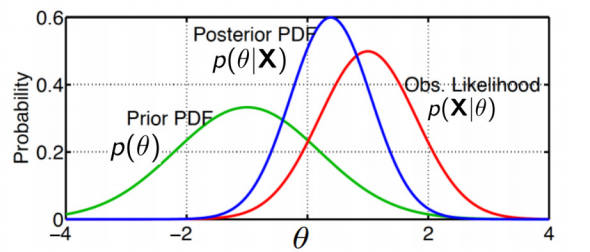
\includegraphics[width=250px]{includes/scribe02/bayesian-inference.png}
			\caption{Visual Look at Bayesian Inference}
		\end{figure}

		In general, the posterior is hard to compute, as $\prob{\vX}$ can be intractable. It is, however, easier if the prior and the likelihood terms and conjugate.

	\end{ssubsection}

	\begin{ssubsection}{Inferring the Full Posterior: Coin-Toss Example}

		The problem is the same as described earlier, and we use the same terms for the likelihood $\para{\tfunc{Bernoulli}{x^n \pipe \theta}}$ and the prior $\para{\tfunc{Beta}{\theta \pipe \alpha, \beta}}$. \br

		The posterior can then be computed as follows

		\begin{align*}
			\prob{\theta \pipe \vX}	&\eq	\frac{\prob{\vX \pipe \theta} \prob{\theta}}{\prob{\vX}} \\
									&\qprop	\prob{\vX \pipe \theta}	\prob{\theta} \\
									&\qprop	\theta^{\sum_{n = 1}^N x^n + \alpha - 1} \para{1 - \theta}^{\beta + N - 1 - \sum_{n = 1}^N x^n}
		\end{align*}

		After normalizing (or through normal inspection), we can say that the posterior is also Beta

		\begin{align*}
			\prob{\theta \pipe \vX}	\eq	\tfunc{Beta}{\theta \pipe \sum_{n = 1}^N x^n + \alpha - 1, \beta + N - 1 - \sum_{n = 1}^N x^n}
		\end{align*}

		Here, the posterior has the same form as the prior (both Beta): \et{property of conjugate priors}

	\end{ssubsection}

	\begin{ssubsection}{Using the Posterior for Prediction}

		We need to predict the probability of getting a head in the next try. Essentially we need to predict the value of $\prob{x = 1 \pipe \vX}$ \br
		
		In order to make predictions, we can use posterior averaging, \et{i.e.} compute the predicted probabilities (of getting a head) over all values of $\theta$ weighted on their posterior probability (Expected Value)

		\begin{align*}
			\prob{x = 1 \pipe \vX}	&\eq	\int_{\theta} \prob{x = 1 \pipe \theta, \vX} \prob{\theta \pipe \vX} d\theta \\
									&\eq	\int_{\theta} \theta \cdot \prob{\theta \pipe \vX} d\theta \\
									&\eq	\E[\prob{\theta \,|\, \vX}]{\theta} \\
									&\eq	\frac{\sum_{n = 1}^N x^n + \alpha}{\alpha + \beta + N}
		\end{align*}

		Hence, $x \sim \tfunc{Bernoulli}{x \pipe \E[\prob{\theta \,|\, \vX}]{\theta}}$ \br

		\note{The predicted distribution doesn't depend on only one point estimate, and is an expectation over the complete distribution}



	\end{ssubsection}<++>

	\begin{ssubsection}{Examples of Conjugate Priors}

		Many pairs of distributions are conjugate to each other such as
		\begin{itemize}
			\item Bernoulli (likelihood) + Beta (prior) $\lra$ Beta posterior
			\item Binomial (likelihood) + Beta (prior) $\lra$ Beta posterior
			\item Multinomial (likelihood) + Dirichlet (prior) $\lra$ Dirichlet posterior
			\item Poisson (likelihood) + Gamma (prior) $\lra$ Gamma posterior
			\item Gaussian (likelihood) + Gaussian (prior) $\lra$ Gaussian posterior
		\end{itemize}

	\end{ssubsection}

\end{ssection}

\end{document}
